\documentclass[12pt,a4paper]{article}

% Packages
\usepackage[utf8]{inputenc}
\usepackage{amsmath,amssymb}
\usepackage{graphicx}
\usepackage{geometry}
\usepackage{listings}
\usepackage{hyperref}

% Page Layout
\geometry{margin=1in}
\setlength{\parindent}{1cm}

% Code Listing Style
\lstset{basicstyle=\ttfamily, frame=single, breaklines=true, captionpos=b}

% Title Page Info
\title{Real Time Signal Processing for Proximity Sensor Data}
\author{Group 04: Uğur ÖZKAN(21050161003), Eren YILMAZ(22050151024), Name3, Name4, Name5}
\date{\today}

\begin{document}

\maketitle
\section{Abstract}

The project aims to develop a dataset for obstacle detection and avoidance in autonomous drones, focusing on the challenging "focus of expansion" where optic flow is minimal. Data was collected using a drone equipped with multiple sensors, including event-based cameras, RGB cameras, radar, and IMU, with ground truth provided by an OptiTrack motion capture system. Experiments were conducted under varying light conditions and with different numbers of obstacles. The dataset comprises 1369 trials and is made available in ROS bag and CSV formats for research in navigation and obstacle avoidance.

\section{Introduction}

The primary challenge addressed is the difficulty autonomous drones face in reliably detecting and avoiding obstacles, especially in dynamic environments with changing lighting. Reliable obstacle detection is crucial for applications like drone delivery, search-and-rescue operations, and autonomous inspections. By addressing these challenges, the dataset promotes innovation in navigation algorithms and machine learning models for real-world scenarios.

\section{Methodology}

This section describes the approaches and techniques used for processing and visualizing multi-sensor data from various sensing modalities.

\subsection{Data Collection and Processing}

The analysis pipeline processes data from five different sensor types:

\begin{itemize}
    \item RGB Camera Data: Video frames are sampled at intervals of 30 frames to obtain key visual information, with a maximum of 5 frames collected for visualization purposes.
    
    \item Dynamic Vision Sensor (DVS): Event-based vision data is processed with parameters DIMX = 240 and DIMY = 180 at 24 FPS. Events are accumulated into frames with polarity-based color coding (red for negative events, blue for positive events).
    
    \item OptiTrack Motion Capture: Position data (x, y, z) and orientation quaternions (a, b, c, d) are collected and time-synchronized with other sensor streams. The data provides ground truth trajectory information.
    
    \item Inertial Measurement Unit (IMU): Linear accelerations and angular velocities are processed in three axes. A moving average filter with window size W = 15 is applied to reduce noise:
    
    \begin{equation}
        x_{filtered}[n] = \frac{1}{W}\sum_{i=0}^{W-1} x[n+i]
    \end{equation}
    
    \item Radar: Two-antenna radar data is processed using Fast Fourier Transform (FFT) analysis. The processing includes:
    \begin{enumerate}
        \item Zero-padding the chirp signals for improved FFT performance
        \item Computing complex FFT for both receive channels
        \item Extracting magnitude and phase information
    \end{enumerate}
\end{itemize}

\subsection{Data Synchronization and Visualization}

All sensor streams are temporally aligned using timestamps normalized to seconds. The visualization pipeline includes:

\begin{enumerate}
    \item Time-series plots for OptiTrack position and orientation data
    \item Filtered and unfiltered IMU measurements visualization
    \item 2D trajectory plot with obstacle locations marked as circles
    \item 3D trajectory visualization with cylindrical obstacles
    \item Radar FFT analysis showing magnitude and phase information
\end{enumerate}

\subsection{Signal Processing Techniques}

Several signal processing methods are employed:

\begin{equation}
    FFT_{radar}(re, im) = \{\mathcal{F}(re + j\cdot im)\}
\end{equation}

The magnitude and phase are computed as:

\begin{equation}
    magnitude = \sqrt{real^2 + imag^2}
\end{equation}

\begin{equation}
    phase = \arctan2(real, imag)
\end{equation}

For the radar processing, we implement:
\begin{itemize}
    \item Zero-padding to improve frequency resolution
    \item FFT shift for centered frequency representation
    \item Complex signal processing for both radar channels
\end{itemize}

\subsection{Coordinate Systems and Transformations}

The system uses multiple coordinate frames:
\begin{itemize}
    \item OptiTrack world coordinate system for absolute positioning
    \item IMU body-fixed coordinate frame for acceleration and angular velocity
    \item Image coordinates for DVS (240×180 pixels) and RGB camera data
\end{itemize}

\subsection{Implementation Details}

The implementation utilizes several Python libraries:
\begin{itemize}
    \item NumPy for numerical computations and array operations
    \item Matplotlib for visualization and plotting
    \item OpenCV (cv2) for RGB video processing
    \item PIL for image processing
    \item SciPy for FFT computations and signal processing
\end{itemize}

The visualization framework is designed to provide comprehensive insight into the sensor fusion dataset, enabling analysis of both spatial and temporal relationships between different sensor modalities.
\section{Data and Implementation}
\textbf{Briefly describe the dataset, preprocessing steps, and Python implementation. Include a code snippet if relevant:}

The dataset contains data from various sensors stored in CSV format. Preprocessing includes filtering noise and normalizing time series. For example, radar data undergoes FFT for frequency domain analysis, while IMU data uses sliding window filters for smoothing.

\begin{lstlisting}[language=Python, caption=Radar Data undergoes FFT]
import numpy as np
from scipy.fft import fft, fftshift

def fft_radar(re, im):
    s1 = fftshift(fft(re))
    s2 = fftshift(fft(im))
    magnitude = np.sqrt(s1.real**2 + s2.imag**2)
    return magnitude

# Load radar sample
radar_data = np.loadtxt('sample_radar.csv', delimiter=',')
real_part = radar_data[:, 1]
imag_part = radar_data[:, 2]
magnitude = fft_radar(real_part, imag_part)

\end{lstlisting}
\section{Results and Discussion}
\textbf{Present findings with graphs or screenshots:}

Using the provided scripts, radar data visualization showcases signal magnitude and phase for obstacle detection. IMU data plots reveal smoothed accelerations and angular velocities, supporting movement dynamics analysis. Below is an example visualization of FFT magnitude for radar data and smoothed IMU signals:

Graphs:

Radar FFT magnitude plot: Peaks indicate obstacle presence at specific distances.
IMU filtered accelerations: Smooth curves represent stability and noise reduction.
\begin{figure}[h!]
    \centering
    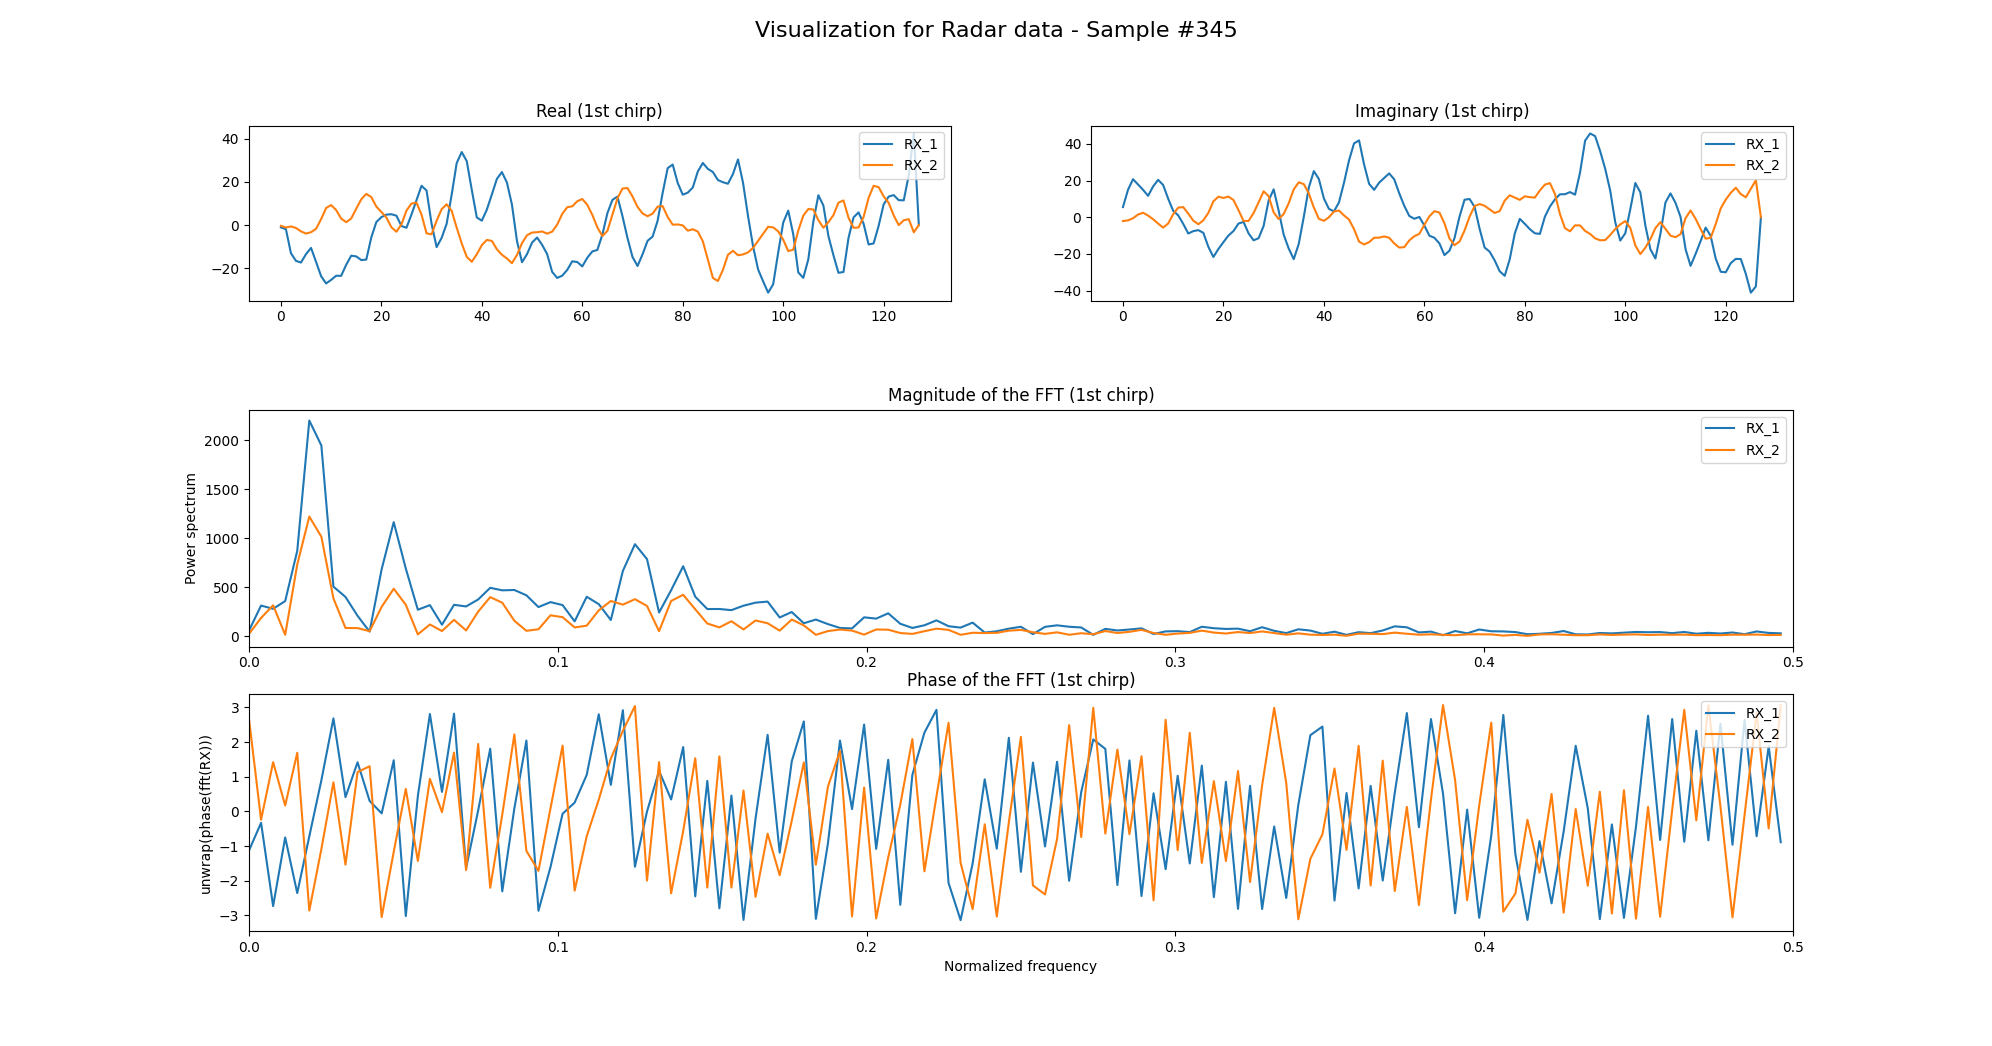
\includegraphics[width=0.8\textwidth]{radar_sample_345.png} 
    \caption{This is the graph of radar sample 345.}
    \label{fig:Radar_sample_345}
\end{figure}

\section{Conclusion}
\textbf{Summarize key outcomes and suggest future improvements.}

\section*{References}
\textbf{List all references, e.g., datasets, websites, or papers.}

\url{https://github.com/JuSquare/ODA_Dataset/tree/master}

\end{document}

